\documentclass[12pt]{article}
\usepackage[margin=1.2in]{geometry}
\usepackage{amsmath}
\usepackage{ctex}
\usepackage{siunitx}
\usepackage{multirow}
\usepackage{bigstrut}
\usepackage{graphicx}
\usepackage{hyperref}
\title{自由落体测重力加速度实验报告}
\author{姓名:宋建宏\,\, 学号:PB21020677\,\, 班级:203院22级5班\\ 日期:2023年4月2日}
\date{}

\begin{document}
\maketitle
\section*{实验目的}
利用自由落体的匀加速直线运动,测量本地的重力加速度,学习调整实验仪器,分析误差来源,使用线性拟合方法分析数据。

\section*{实验原理}
对于自由落体运动,由牛顿第二定律得
\begin{equation}\label{1}
    h=\frac{1}{2}gt^2
\end{equation}

但是总时间\(t\)不容易测准,我们选择测量其中一段的时间和距离:
光电门1的位置固定,即小球通过光电门1时的速度$v_0$保持不变,小球通过光电门1与光电门2的高度差为$h_i$,时间差为$t_i$,
改变光电门2的位置,则有:
$$
    \begin{gathered}
        h_1=v_0 t_1+\frac{1}{2} g \mathrm{t}_1^2 \\
        h_2=v_0 t_2+\frac{1}{2} g \mathrm{t}_2^2 \\
        \cdots \\
        h_i=v_0 t_i+\frac{1}{2} g \mathrm{t}_i^2
    \end{gathered}
$$
两端同时除以 $t_i$ :
$$
    \begin{gathered}
        \overline{v_1}=\frac{h_1}{t_1}=v_0+\frac{1}{2} g t_1 \\
        \overline{v_2}=\frac{h_2}{t_2}=v_0+\frac{1}{2} g t_2 \\
        \cdots \\
        \overline{v_i}=\frac{h_i}{t_i}=v_0+\frac{1}{2} g t_i
    \end{gathered}
$$
测出系列 $h_i 、 t_i$, 利用线性拟合即可求出当地的重力加速度 $g$ 。

\section*{实验器材}
\

卷尺、自由落体装置。

\section*{分析与讨论}

\subsection*{数据处理}
本次实验记录8组不同的高度差,每个高度差通过三组实验测量时间,每组实验的数据记录如下:
% Table generated by Excel2LaTeX from sheet 'Sheet1'
\begin{table*}[htbp]
    \centering
    \begin{tabular}{|r|r|r|r|r|r|r|}
        \hline
        \multicolumn{1}{|c|}{\multirow{2}[4]{*}{ 组别}} & \multicolumn{1}{c|}{高度差 } & \multicolumn{4}{c|}{时间差$\Delta t /\SI{}{ms}$} & \multicolumn{1}{l|}{平均速度} \bigstrut                                                                                              \\
        \cline{3-6}                                   & $\Delta h/\SI{}{cm}$      & \multicolumn{1}{l|}{第一次}                      & \multicolumn{1}{l|}{第二次}            & \multicolumn{1}{l|}{第三次} & \multicolumn{1}{l|}{平均} & $\overline{v}/(\SI{}{m/s})$ \bigstrut \\
        \hline
        1                                             & 20.07                     & 101.3                                         & 101.6                               & 101.7                    & 101.53                  & 1.977 \bigstrut                       \\
        \hline
        2                                             & 27.87                     & 131.5                                         & 131.5                               & 131.5                    & 131.50                  & 2.119 \bigstrut                       \\
        \hline
        3                                             & 35.77                     & 158.5                                         & 158.5                               & 158.5                    & 158.50                  & 2.257 \bigstrut                       \\
        \hline
        4                                             & 43.90                     & 183.2                                         & 183.3                               & 183.3                    & 183.27                  & 2.395 \bigstrut                       \\
        \hline
        5                                             & 51.83                     & 206.9                                         & 207.0                               & 206.9                    & 206.93                  & 2.504 \bigstrut                       \\
        \hline
        6                                             & 59.97                     & 229.0                                         & 229.1                               & 229.1                    & 229.07                  & 2.618 \bigstrut                       \\
        \hline
        7                                             & 67.83                     & 250.1                                         & 250.1                               & 250.1                    & 250.10                  & 2.712 \bigstrut                       \\
        \hline
        8                                             & 75.91                     & 269.6                                         & 269.6                               & 269.6                    & 269.60                  & 2.817 \bigstrut                       \\
        \hline
    \end{tabular}%
\end{table*}%

线性拟合
如下图
\begin{figure*}[htbp]
    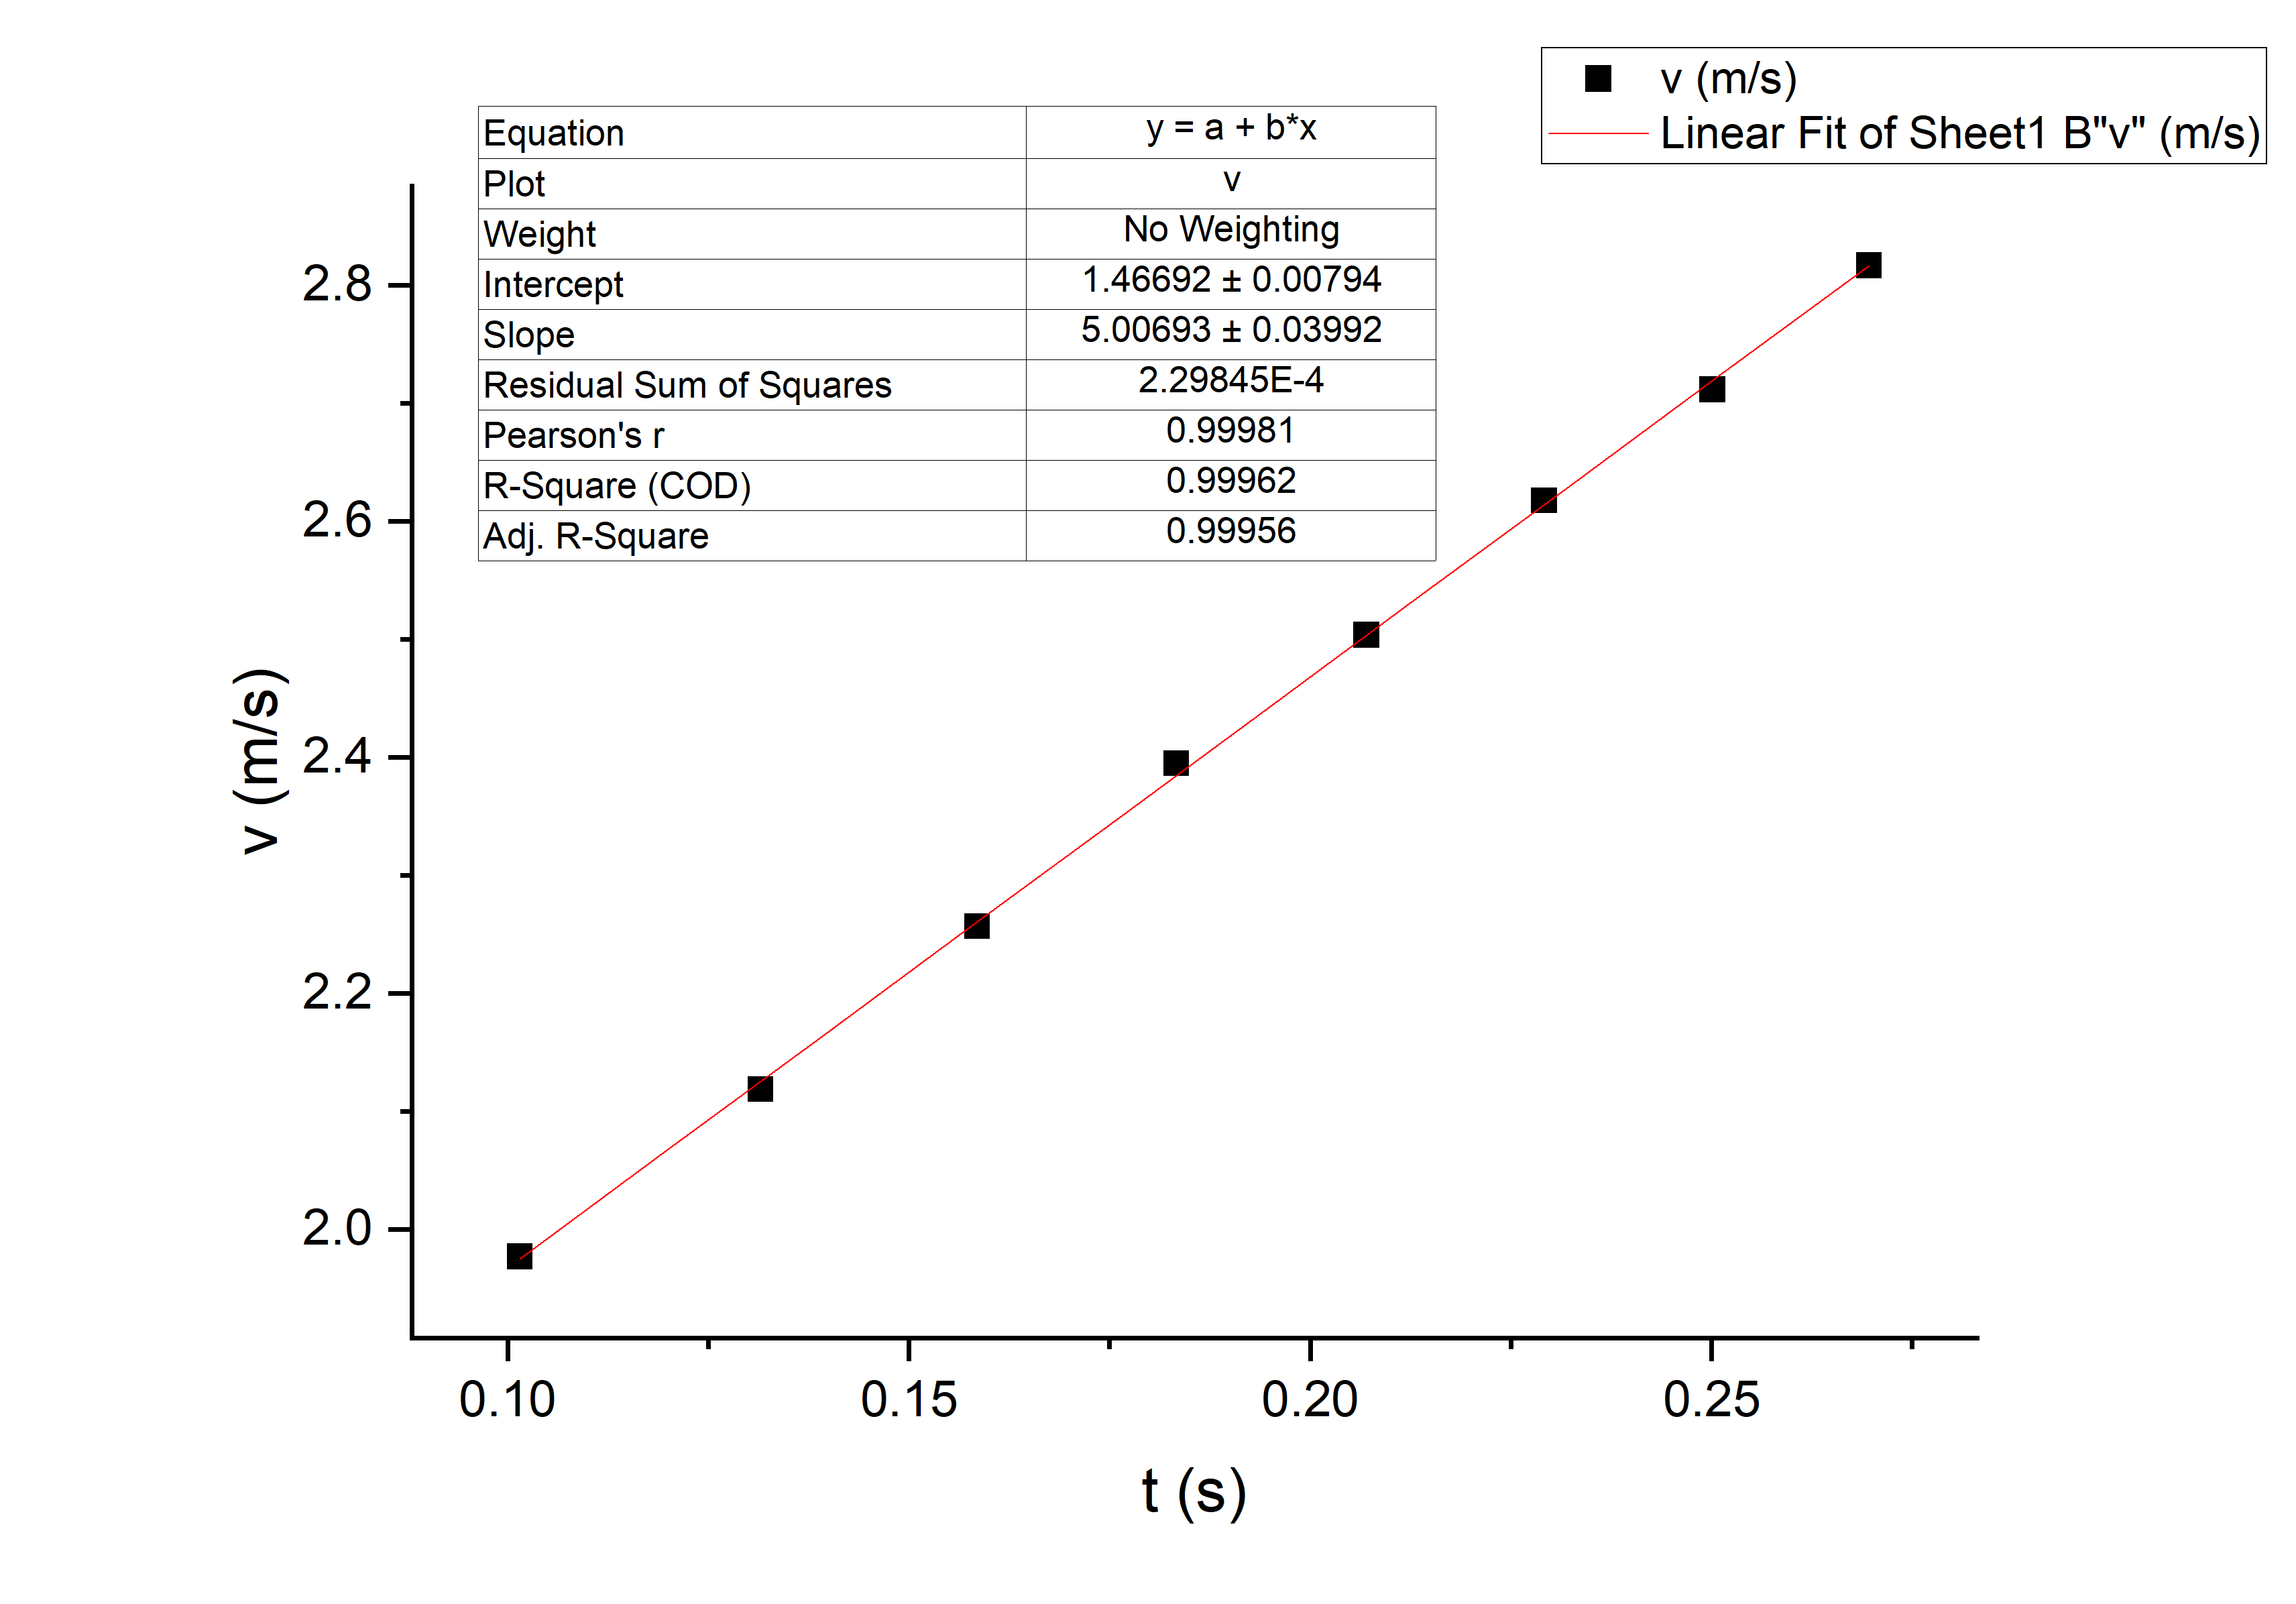
\includegraphics[scale=0.5]{graph.png}
\end{figure*}

得\(v=5.00693t+1.46692(\SI{}{m/s})\),线性相关系数 \(r=0.99981\),于是得重力加速度
\[g=2\times 5.00693=\SI{10.01386}{m/s^2}\]



\subsection*{误差分析}

合肥地区重力加速度参考值为$g_0=\SI{9.7947}{m/s^2}$,因此实验相对误差为
\[\delta =\frac{|g-g_0|}{g_0}=2.8\%\]
误差较大。

可能的误差来源:小球中心与光电门有偏离,导致测量时间误差;光电门间距测量误差等。



\section*{思考题}
\begin{enumerate}
    \item 在实际工作中, 为什么利用\eqref{1}式很难精确测量重力加速度$ g$?
    
    答:由于一些系统误差的存在,比如仪器释放的过程中磁力并非迅速衰减等,导致的时间误差等,导致用时$ t $很难测量精准, 因此使用这种方法, 测
    量$ t $的误差比较大; 同时, 由于小球的尺寸、光电门的位置等的原因, 使得小球下
    落的高度$ h $也很难测准。 因此该公式很难精确测量重力加速度 $g$.

\item 为了提高测量精度, 光电门 1 和光电门 2 的位置应如何选取?

答: 光电门 1 大约置于悬挂点下 10cm 处, 并在测量过程中保持不动; 光电门
2 在光电门 1 下方, 距离从 20cm 到 80cm 左右比较合适, 应该在这个范围内, 多
次调节光电门 2 的位置, 从而获得多组数据。 两个光电门不应该距离太近, 否则
测出的区间平均速度不够准确; 距离太远则会超出立柱允许的范围, 同时空气阻
力的影响也会增大。

\item 利用本实验装置, 你还能提出其他测量重力加速度$ g $的实验方案吗?

答: 类似于用单摆测量重力加速度, 可以使用光电门测量摆的周期: 
将摆的顶端悬挂后, 调整一个光电门的位置使得小球处于最底端时, 正好
可以遮挡住光电门的光路。 释放小球, 根据光电门的时间读数可以计算出小球摆
动的周期。
\end{enumerate}



\end{document}